\chapter{Introduction}\label{Ch:Introduction}

% Motivation
\section{Sponsor}
Advanced Micro Devices, Inc. (AMD) is an American multinational semiconductor company based in Santa Clara, California, that develops computer processors and related technologies for business and consumer markets. AMD's main products include microprocessors, motherboard chipsets, embedded processors and graphics processors for servers, workstations and personal computers, and embedded systems applications. AMD is interested in developing powerful hardware devices and software for machine learning tasks. The results from this project will provide insights for improving hardware efficiency needed for deep reinforcement learning algorithms. 

\section{Motivation}
% % Black-box image
% \begin{figure}[h!]
% \centering
% 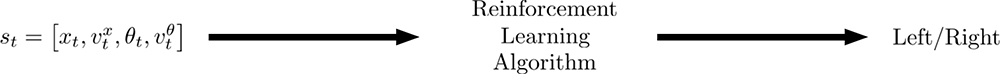
\includegraphics[scale=0.35]{Graphics/black_box_small.png}
% \caption[Reinforcement Learning Representation]{The black box is a representation of the reinforcement learning algorithm. The algorithm takes in a state from the environment, which passes through a black box to output the optimal action in the current state.}
% \label{fig:black_box}
% \end{figure}

Supervised machine learning approaches operate in distinct modes of training and inference. During training, an algorithm is shown labeled data and learns a representation of the underlying distribution of the data. After training, the model can be deployed to infer predictions based on the information it learns during training. However, supervised machine learning approaches are limited because they require labeled data, and labeled data is not always available. 

Reinforcement learning is a goal-oriented approach that is fundamentally different from supervised machine learning. The objective of reinforcement learning is to provide a means for an agent to continually learn while dynamically interacting with an environment. As the agent performs actions within the environment, it receives feedback through rewards and learns new behavior. The goal of the algorithm is to find the optimal actions at each given state. This is distinct from typical approaches in artificial intelligence, where an algorithm must first learn by viewing examples of a task being performed before it is capable of making predictions for this same task. 

However, there are many challenges to overcome in the field of reinforcement learning. First, reinforcement learning fails in area where it requires long-term strategy. Second, reinforcement learning requires a huge amount of training time and experience. Third, reinforcement learning is not robust to adjust to perturbations in the environment. This impediment is the main focus of this project. The goal is to investigate the sensitivity of reinforcement learning algorithms and try to develop a robust algorithm that can adapt to changes in the environment.

\section{Problem Statement}
This project focused on improving the flexibility of reinforcement learning algorithms, allowing them to adapt to perturbations in the environment. We explored common frameworks and algorithms in reinforcement learning and investigated techniques to reduce the power consumption and latency of the deployed model without compromising the accuracy of the system. We investigated the effects of enriching the feedback received by the agent to guide it towards more effective learning. Moreover, analysis of model efficiency revolved around characterizing the influence of hyperparameters and sensitivity to hardware devices.

%Reinforcement learning agents learn by exploring their environment 
%freely and receiving rewards for ideal behavior. A natural venue
%that provides such a sandbox is computer games. Computer games have well-defined environment, action, and reward. These games also do not require a physical device to interact with the environment. We can easily change the environment by varying the parameters of the game settings. Computer games fulfill the criteria for our exploration. We will particularly focus on a car racing game, which is potentially applicable to autonomous cars.

\section{Approach}
Computer games were used as a sandbox to explore the sensitivity of reinforcement learning algorithms. There are several advantages with using computer games: first, computer games have well-defined rules; second, they provide an efficient avenue for collecting data; third, the environment can be easily changed in order to induce perturbations. In particular, our investigations focused on an unsolved car racing challenge provided by the OpenAI Gym \cite{brockman2016openai}. The environment in the car racing game is interesting due to its application to autonomous cars. 

First, we implemented basic reinforcement learning algorithm with success in simple classic control games. Next, we implemented reinforcement learning algorithm incorporating deep learning, which produced promising results on a few classic control games and the Atari Breakout game. We then implemented deep Q-learning on the car racing game and explored the effect of reward clipping and regularization on performance. Lastly, we explored data compression in inputs to investigate how to reduce the storage required by the algorithm.

\section{Overview}
In this report, we will first explain the mathematical foundations of reinforcement learning in Chapter \ref{Ch:Reinforcement Learning}. Then we will focus on Q-learning and its implementation in Chapter \ref{Ch:Q-Learning-Representations}. We will present some of our successful results on some of the simple classic control and Atari games in Chapter \ref{Ch:ResultsPrelim}. We will discuss the results and findings while attempting to solve a car racing game in Chapter \ref{Ch:ResultsCarRacing} and \ref{Ch:Analyze}. Lastly, in Chapter \ref{Ch:FutureWork}, we provide ideas for future works needed to be done to make the algorithm more robust.

\endinput

